%for a more compact document, add the option openany to avoid
%starting all chapters on odd numbered pages
\documentclass[12pt]{cmuthesis}

% This is a template for a CMU thesis.  It is 18 pages without any content :-)
% The source for this is pulled from a variety of sources and people.
% Here's a partial list of people who may or may have not contributed:
%
%        bnoble   = Brian Noble
%        caruana  = Rich Caruana
%        colohan  = Chris Colohan
%        jab      = Justin Boyan
%        josullvn = Joseph O'Sullivan
%        jrs      = Jonathan Shewchuk
%        kosak    = Corey Kosak
%        mjz      = Matt Zekauskas (mattz@cs)
%        pdinda   = Peter Dinda
%        pfr      = Patrick Riley
%        dkoes = David Koes (me)

% My main contribution is putting everything into a single class files and small
% template since I prefer this to some complicated sprawling directory tree with
% makefiles.

% some useful packages
\usepackage{times}
\usepackage{fullpage}
\usepackage{graphicx}
\usepackage{amsmath}
\usepackage{cite}
\usepackage[numbers,sort]{natbib}
\usepackage[pageanchor=true,plainpages=false, pdfpagelabels, bookmarks,bookmarksnumbered,
%pdfborder=0 0 0,  %removes outlines around hyper links in online display
]{hyperref}
\usepackage{setspace}
\usepackage{subfigure}
\usepackage{titlesec}
\titleformat{\chapter}[hang] 
{\normalfont\LARGE\bfseries}{\chaptertitlename\ \thechapter:}{1em}{}

% Approximately 1" margins, more space on binding side
%\usepackage[letterpaper,twoside,vscale=.8,hscale=.75,nomarginpar]{geometry}
%for general printing (not binding)
\usepackage[letterpaper,twoside,vscale=.8,hscale=.75,nomarginpar,hmarginratio=1:1]{geometry}

% Provides a draft mark at the top of the document. 
\draftstamp{\today}{DRAFT}

\begin {document} 
\frontmatter

%initialize page style, so contents come out right (see bot) -mjz
\pagestyle{empty}

\title{ %% {\it \huge Thesis Proposal}\\
{\bf PROPOSAL: Unsupervised Guitar String Classification for Tablature Transcription}}
\author{Jonathan Michelson}
\date{April 2017}
\Year{2017}
\trnumber{}

\committee{
Dr. Richard Stern, Dr. Tom Sullivan \\
}

\support{}
\disclaimer{}

% copyright notice generated automatically from Year and author.
% permission added if \permission{} given.

%\keywords{Stuff, More Stuff}

\maketitle

%\begin{dedication}
%For my dog
%\end{dedication}

\pagestyle{plain} % for toc, was empty

%% Obviously, it's probably a good idea to break the various sections of your thesis
%% into different files and input them into this file...

%\doublespacing
%\begin{abstract}
%Guitar tablature transcription (brief explanation) is a commonly used music notation standard that could benefit from automation. Previous work solves this task in a framework that requires prior information about the guitar. Here, an unsupervised offline solution is introduced. Inharmonicity estimates extracted from isolated guitar notes naturally segregate into semi-linear formations determined by its sourced string. The inharmonicities are modeled with a linear regression mixture, and optimized with expectation maximization. 
%\end{abstract}
%\singlespacing

%\begin{acknowledgments}
%My advisor is cool.
%\end{acknowledgments}



%\tableofcontents
%\listoffigures
%\listoftables

\mainmatter

%% Double space document for easy review:
%\renewcommand{\baselinestretch}{1.66}\normalsize

% The other requirements Catherine has:
%
%  - avoid large margins.  She wants the thesis to use fewer pages, 
%    especially if it requires colour printing.
%
%  - The thesis should be formatted for double-sided printing.  This
%    means that all chapters, acknowledgements, table of contents, etc.
%    should start on odd numbered (right facing) pages.
%
%  - You need to use the department standard tech report title page.  I
%    have tried to ensure that the title page here conforms to this
%    standard.
%
%  - Use a nice serif font, such as Times Roman.  Sans serif looks bad.
%
% Other than that, just make it look good...
\chapter{Proposal}
\noindent
\textbf{Background} - The guitar is a widely popular instrument whose neighboring strings' pitch ranges overlap. Consequently, a given musical phrase can usually be realized in a few different ways by a performer. Conventional music scores represent passages as notes and chords, and therefore leave fretboard position ambiguous. Tablature is an alternative music notation for guitarists that doesn't suffer from the one-to-many mapping of scores. Automating its tedious annotation process is an interesting MIR problem with applications in music education.

\noindent
\textbf{Previous Work} - Inharmonicity seems to be a key feature in automatic string discrimination. It relates the physical properties of a vibrating string -- Young's modulus, diameter, length, tension -- to the degree of its harmonics' deviations from their ideal frequency locations: integer multiples of their fundamental. Estimation typically involves searching a note's spectrum for peaks in the vicinity of multiples of the fundamental, then cataloguing located peaks' deviations from their ideal locations, and fitting a polynomial -- one of whose coefficients corresponds to a good estimate of the inharmonicity -- to the deviations curve. Barbancho~\cite{barbanchoi2012} achieves good tablature transcription using open-strings' inharmonicities and checking unknown notes' inharmonicities against those of string candidates. In various supervised classification approaches~\cite{abesser2012, kehling2014, dittmar2013}, the authors achieve good string transcription after training on standard-tuning guitar audio and using inharmonicity as one of their features.

\noindent
\textbf{Missing Science} - Previous inharmonicity-based transcription systems require prior information for their success: Barbancho~\cite{barbanchoi2012} requires seeding the system with known open strings' inharmonicities, and Abesser, Kehling, and Dittmar~\cite{abesser2012, kehling2014, dittmar2013} require labeled training data. Additionally, it's unclear how these systems will perform when tested against guitars in some known but non-standard tuning.

\noindent
\textbf{Proposed Solution} - An unsupervised approach could address the discussed limitations. We propose the following unsupervised pipeline: (1) inharmonicity estimation, using the polynomial-fit approach discussed above; (2) linear regression mixture modeling~\cite{faria2010}, which will be solved using EM; (3) string clustering, where we simply assign each note to the line that best explains it.

\noindent
\textbf{Pilot Results} - Figure \ref{fig:beta} shows best-case results for inharmonicity estimation and plotting. In Figure~\ref{fig:em}, current best-case results for linear regression estimation are shown. Classification F-scores by string are $[1.0, 1.0, 0.89, 0.8, 0.57, 1.0]$. Average F-score $ = 0.88$.

\begin{figure}[h]
\centering
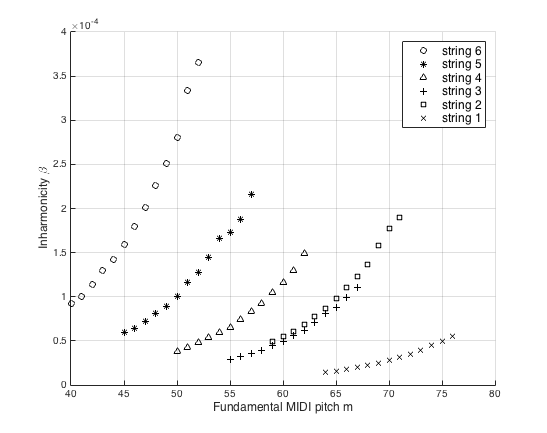
\includegraphics[scale=.6]{beta-v-midi.png}
\caption{Inharmonicities $\beta$ (y-axis) vs. MIDI note number (x-axis). The six different colors correspond to the six string labels E2, A2, D3, G3, B3, E4. This electric guitar recording enumerated the 78 notes between E2 and E5 inclusive in standard-tuning.}
\label{fig:beta}
\end{figure}

\begin{figure}[h]
\centering
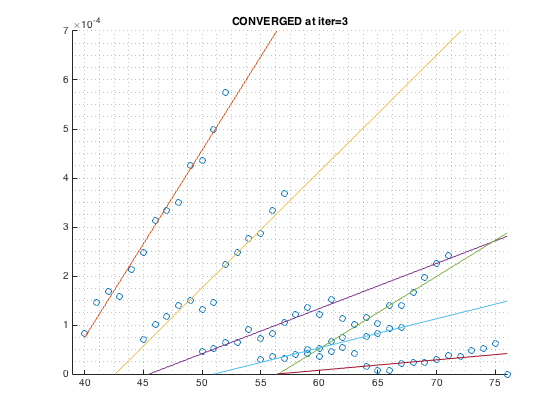
\includegraphics[scale=0.6]{em.png}
\caption{Converged EM estimate of the linear regressions. Same axes as fig. \ref{fig:beta}.}
\label{fig:em}
\end{figure}

\noindent
\textbf{Work to be Done} - \textit{Core System Development}: (1) Finish method to determine number of mixtures present; (2) Finish method to initialize linear regression estimates -- currently done with linear regression on spectral clustering results~\cite{shi2000,ng2001}; (3) Finish mapping from string clusterings to fretboard position. \textit{Experiments}: Run system on dataset (discussed in next section), vary the following experiment parameters and observe effect on performance: (1) mixture number determination method parameters, (2) linear regression initialization method parameters, (3) linear regression parameters (variance, mixing probabilities), (4) dataset attributes (number/density of notes, number of strings)

\noindent
\textbf{Evaluation Criteria} - \textit{Dataset}: subset of the RWC Music Instrument database: clean, isolated, monophonic plucks of frets 0-12 on strings 1-6 of a Fender Stratocaster, Aria PE, and Ibanez Artcore, each of which has the following recording iterations: plucking style (finger, plectrum), dynamic level (soft, medium, loud)~\cite{goto2003}. We'll also personally record four tuning iterations (standard, whole-step down, whole-step up, DADGAD) of frets 0-12 on strings 1-6 of an Ibanez RG for assessment of this approach's tuning invariance. String-fret labels are known in both datasets. \textit{Evaluation}: String classification F-scores and confusion matrices.

\noindent
\textbf{Deliverables} - Experiment results, thesis (draft + final).

\noindent
\textbf{Timetable} - Proposal final: 4/10; thesis draft: 5/1; thesis final: 5/15.

%\appendix
%\include{appendix}

\backmatter

%\renewcommand{\baselinestretch}{1.0}\normalsize

% By default \bibsection is \chapter*, but we really want this to show
% up in the table of contents and pdf bookmarks.
\renewcommand{\bibsection}{\chapter{\bibname}}
%\newcommand{\bibpreamble}{This text goes between the ``Bibliography'' header and the actual list of references}
\bibliography{mybib} %your bib file
\bibliographystyle{plainnat}


\end{document}
